%!TEX program = xelatex
\documentclass[12pt, b5paper]{article}
\usepackage{ctex}

\usepackage{geometry}
\geometry{b5paper,left=2cm,right=1cm,top=2.5cm,bottom=2.5cm}
\usepackage{chemformula} %化学公式宏包
\usepackage[version=4]{mhchem} %化学公式宏包
\usepackage{siunitx} %数字，单位宏包
\sisetup{
	separate-uncertainty = true,
	inter-unit-product = \ensuremath{{}\cdot{}}
} %单位间加小圆点
\usepackage{tikz} %Tikz绘图包
\usetikzlibrary{cd}
\usetikzlibrary{chains}
\usetikzlibrary{arrows}
\usetikzlibrary{arrows.meta} %画箭头
\usetikzlibrary{commutative-diagrams} %交换图
\usetikzlibrary{positioning,automata}
\usepackage[all]{xy}
\usepackage{booktabs} %三线表
\usepackage{multirow} %合并单元格
\usepackage{makecell} %表格内强制换行
\usepackage{array}
\usepackage{booktabs} %控制表格行高
\usepackage{colortbl}  %彩色表格需要加载的宏包
\usepackage{amsmath}
\usepackage{unicode-math}
\usepackage{fontspec} %字体
\newcommand*{\cred}{\textcolor{red}}

\setmainfont{Times New Roman}
\setmathfont{XITS Math}

\setlength{\parindent}{0pt} %无缩进
\usepackage{setspace}
\usepackage{fancyhdr} %设置页码
\usepackage{lastpage} %获取总页数
\pagestyle{fancy} %fancyhdr宏包新增的页面风格
\renewcommand\headrulewidth{0pt} %取消页眉中的装饰分割线
\fancyhf{}
\cfoot{\footnotesize 第 \thepage\ 页(共 \pageref{LastPage}页)}%当前页 of 总页数

\begin{document}
\begin{spacing}{1.625}

\centerline{{\huge 河北农业大学课程考试试卷}}

\centerline{\large 2022-2023学年第\underline{\ 1\ }学期}

考试科目：\underline{化学反应工程} \hfill 姓名：\underline{ \qquad \qquad} \hfill 学号：\underline{ \qquad \qquad \qquad \qquad}

学院：\underline{理工学院} \hfill 专业班级：\underline{\qquad \qquad \qquad \qquad} \hfill 卷别：\cred{B} \hfill 考核方式：\cred{开卷}

\bigskip


1. 简答题(15分)

简述固定床反应器的优缺点。

\bigskip
\bigskip

2. 简答题(15分)

简述工业反应器的主要操作方式及其特点。

\bigskip
\bigskip

3. 简答题(16分)

谈谈你对《反应工程》的理解。

\bigskip
\bigskip

4. 读图题(24分)

\begin{figure}[htpb]
	\centering
	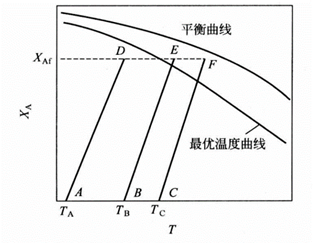
\includegraphics[width=.5\linewidth]{figures/fig3.png}
\end{figure}
上图为某可逆放热反应的转化率与温度的关系。回答以下问题：

(1) A、B、C三点反应速率大小比较？说明原因。

(2) D、E、F三点反应速率大小比较？说明原因。

(3) 对于此类型反应，如何选择最佳操作温度？分别从等温操作、变温操作、绝热操作三种操作方式加以说明。

\bigskip
\bigskip

5. 计算题(30分)

一活塞流反应器和一全混流反应器用两种方式串联。

(a) 活塞流反应器在前 ， 全混流反应器在后

(b) 全混流反应器在前 ， 活塞流反应器在后

今分别在其中进行一级不可逆反应 ：\ch{A -> R}。

己知 $k = 2 \mathrm{h}^{-1}$ ，物料在每个反应器中的停留时间均为 30 min ， $c_\mathrm{A0}=10\si{mol/L}$
，若两反应器温度相同，反应过程中物料密度基本不变，试计算两种情况下的出口浓度 。

\end{spacing}
\end{document}
